% ==============================================================================
% DevOS Research Paper Template - IEEE/ACM Conference Format
% ==============================================================================
% Compile with: pdflatex main.tex -> bibtex main -> pdflatex main.tex (x2)
% Or use Overleaf: Upload this entire folder as a project
% ==============================================================================

\documentclass[conference,10pt,caption=false]{IEEEtran}

% --------------------------------------------------------------
% PACKAGES
% --------------------------------------------------------------
\usepackage[utf8]{inputenc}
\usepackage[T1]{fontenc}
\usepackage{graphicx}
\usepackage{booktabs}
\usepackage{amsmath}
\usepackage{amssymb}
\usepackage{algorithm}
\usepackage{algorithmicx}
\usepackage{algpseudocode}
\usepackage{listings}
\usepackage{xcolor}
\usepackage{tabularx}  % Added for better table formatting
\usepackage{hyperref}
\usepackage{cleveref}
\usepackage{subcaption}
\usepackage{multirow}
\usepackage{makecell}
\usepackage{balance}   % For balancing columns on last page
\usepackage{tikz}
\usetikzlibrary{shapes, arrows.meta, positioning, calc, fit, backgrounds, shadows} % Added shadows
\usepackage{xspace}    % For \xspace in \devos command
\usepackage{pifont}    % For \ding and \checkmark symbols
\usepackage{enumitem}  % For compact lists
\usepackage{footnote}  % For table footnotes
\usepackage{textcomp}  % For \textcircled in figure caption

% --------------------------------------------------------------
% HYPERREF SETUP
% --------------------------------------------------------------
\hypersetup{
    colorlinks=true,
    linkcolor=blue,
    filecolor=magenta,
    urlcolor=cyan,
    citecolor=blue,
    pdfauthor={Harshit, Ravent, Isha},
    pdftitle={DevOS: A Self-Healing AI Development Environment},
    pdfsubject={B.Tech Minor Project - Self-Healing Development Environment},
    pdfkeywords={Self-Healing Systems, AI-Assisted Development, Automated Diagnosis, Sandbox Execution, Verified Recovery, LLM Safety}
}

% --------------------------------------------------------------
% LISTINGS SETUP (for code snippets)
% --------------------------------------------------------------
\definecolor{codegreen}{rgb}{0,0.6,0}
\definecolor{codegray}{rgb}{0.5,0.5,0.5}
\definecolor{codepurple}{rgb}{0.58,0,0.82}
\definecolor{backcolour}{rgb}{0.95,0.95,0.92}

\lstdefinestyle{mystyle}{
    backgroundcolor=\color{backcolour},
    commentstyle=\color{codegreen},
    keywordstyle=\color{magenta},
    numberstyle=\tiny\color{codegray},
    stringstyle=\color{codepurple},
    basicstyle=\ttfamily\footnotesize,
    breakatwhitespace=false,
    breaklines=true,
    captionpos=b,
    keepspaces=true,
    numbers=left,
    numbersep=5pt,
    showspaces=false,
    showstringspaces=false,
    showtabs=false,
    tabsize=2,
    frame=single,
    framerule=0.5pt
}

\lstset{style=mystyle}

% --------------------------------------------------------------
% CUSTOM COMMANDS & BADGES
% --------------------------------------------------------------
\newcommand{\devos}{\textsc{DevOS}\xspace}
\newcommand{\todo}[1]{\textcolor{red}{[TODO: #1]}}
\newcommand{\rev}[1]{\textcolor{blue}{#1}}
\newcommand{\etal}{\textit{et al.}\xspace}
\newcommand{\ie}{\textit{i.e.}\xspace}
\newcommand{\eg}{\textit{e.g.}\xspace}
\newcommand{\etc}{\textit{etc.}\xspace}
\newcommand{\cf}{\textit{cf.}\xspace}
\newcommand{\circled}[1]{\raisebox{.5pt}{\textcircled{\raisebox{-.9pt}{\scriptsize #1}}}}

% Table Badges
\newcommand{\badgeLow}{\tikz[baseline=-0.4ex]\node[fill=green!60!black, text=white, rounded corners=2pt, inner sep=2.5pt, font=\sffamily\tiny\bfseries]{LOW};}
\newcommand{\badgeMed}{\tikz[baseline=-0.4ex]\node[fill=orange!80!black, text=white, rounded corners=2pt, inner sep=2.5pt, font=\sffamily\tiny\bfseries]{MEDIUM};}
\newcommand{\badgeHigh}{\tikz[baseline=-0.4ex]\node[fill=red!70!black, text=white, rounded corners=2pt, inner sep=2.5pt, font=\sffamily\tiny\bfseries]{HIGH};}

\newcommand{\badgeAllow}{\tikz[baseline=-0.4ex]\node[fill=green!60!black, text=white, rounded corners=2pt, inner sep=2.5pt, font=\sffamily\tiny\bfseries]{ALLOW};}
\newcommand{\badgeReq}{\tikz[baseline=-0.4ex]\node[fill=orange!80!black, text=white, rounded corners=2pt, inner sep=2.5pt, font=\sffamily\tiny\bfseries]{REQ\_APPROVAL};}
\newcommand{\badgeBlock}{\tikz[baseline=-0.4ex]\node[fill=red!70!black, text=white, rounded corners=2pt, inner sep=2.5pt, font=\sffamily\tiny\bfseries]{BLOCK};}

\newcommand{\vpass}{\textcolor{green!60!black}{\textbf{\texttt{VERIFIED}}}}
\newcommand{\vfail}{\textcolor{red!60!black}{\textbf{\texttt{FAILED}}}}
\newcommand{\vna}{\textcolor{gray}{\textbf{\texttt{N/A}}}}

% --------------------------------------------------------------
% METADATA
% --------------------------------------------------------------
\title{DevOS: A Self-Healing AI Development Environment\\for Automated Project Recovery}

\author{
\IEEEauthorblockN{Harshit\IEEEauthorrefmark{1}, Ravent\IEEEauthorrefmark{1}, Isha\IEEEauthorrefmark{1}}
\IEEEauthorblockA{
\IEEEauthorrefmark{1}Vivekananda Institute of Professional Studies - Technical Campus\\
Affiliated to GGSIP University, Delhi\\
\{01717702723, 04417702723, 03717702723\}@vips.edu
}
}

% --------------------------------------------------------------
% DOCUMENT START
% --------------------------------------------------------------
\begin{document}

\maketitle

% ==============================================================================
% ABSTRACT
% ==============================================================================
\begin{abstract}
Modern software projects fail not from single bugs but from \textit{environmental drift}---the progressive divergence between code, dependencies, environment configuration, databases, ports, services, and runtime state. While recent advances in LLM-based automated program repair~\cite{llm-apr-survey-2025} and autonomous software engineering agents~\cite{swe-bench, swe-agent, devin} have dramatically improved \textit{code-level} bug fixing, they assume a correctly configured environment. No existing tool detects, diagnoses, and repairs the environmental failures that prevent a project from running in the first place. Worse, when granted shell access, these agents operate without safety guarantees: no policy enforcement, no sandboxed execution, no verification, and no rollback~\cite{security-audit, llm-code-security}.

We present \devos, a self-healing AI development environment that unifies project understanding, diagnosis, safe execution, and verified recovery into a single deterministic loop: \textbf{Understand $\to$ Diagnose $\to$ Protect $\to$ Execute $\to$ Verify $\to$ Recover}. \devos imports a project's complete manifest (dependencies, configuration, compose services, database schema, Git state), runs a multi-layer \textit{Project Doctor} to produce evidence-ranked findings, generates a typed recovery plan via a rule-based AI planner, enforces a deterministic policy engine with mandatory approval for risky actions, executes approved steps in a resource-bounded Docker sandbox, and verifies the result through a build/test/health/log verification ladder---automatically rolling back on failure.

Our prototype targets a React + Node.js + PostgreSQL reference stack and automatically repairs eight failure classes across nine end-to-end scenarios, demonstrating 100\% success on reparable failures with automatic rollback on unverifiable changes. The system comprises 245 backend tests, a React/TypeScript web UI, and a terminal CLI, all open-source.
\end{abstract}

% ==============================================================================
% KEYWORDS
% ==============================================================================
\begin{IEEEkeywords}
Self-Healing Systems, AI-Assisted Software Engineering, Automated Program Repair, Sandbox Execution, Verified Recovery, Developer Environment, Policy Enforcement, Docker Sandbox, LLM Safety Guardrails
\end{IEEEkeywords}

% ==============================================================================
% 1. INTRODUCTION
% ==============================================================================
\section{Introduction}
\label{sec:intro}

% --- Context & Problem ---
Modern software development depends on a complex interplay of components: source code, declared dependencies, environment configuration, background services, database state, network ports, and host-level processes~\cite{docker2026security, linux2026proc}. A failure in any one dimension---missing \texttt{DATABASE\_URL}, an uninstalled \texttt{npm} package, a port already in use, a stopped PostgreSQL container, or a drifted schema---prevents the application from running. Critically, these failures \textit{compound}: a missing environment variable can hide a database authentication error, which in turn masks a missing schema.

Developers today must manually switch between a code editor, terminal, container tooling (\texttt{docker compose}), database client (\texttt{psql}), log files, version control (\texttt{git}), and increasingly, an AI chat assistant. Each tool sees only a narrow slice of the project state, leaving the developer to mentally reconstruct the full picture and identify the root cause. This manual correlation is slow, error-prone, and does not scale with project complexity.

% --- Gap in Existing Tools ---
The 2024--2025 explosion in AI-assisted software engineering has produced impressive results in \textit{code-level} repair. LLM-based APR systems~\cite{llm-apr-survey-2023, llm-apr-survey-2025} fix bugs by generating patches from issue descriptions. Autonomous agents like SWE-agent~\cite{swe-agent}, AutoCodeRover~\cite{autocoderover}, and Devin~\cite{devin} resolve real-world GitHub issues end-to-end, achieving over 50\% on the SWE-bench benchmark~\cite{swe-bench, swebench-verified}. Yet all of these systems share a critical assumption: \textit{the environment is correctly configured}. They operate on the code inside an already-working development setup.

When the environment itself is broken---wrong \texttt{.env} values, missing \texttt{node\_modules}, a dead database container, a port collision---these tools cannot help. Moreover, AI coding assistants (GitHub Copilot~\cite{copilot}, Cursor~\cite{cursor}, Codeium~\cite{codeium}, Claude Code~\cite{claude-code}) that offer terminal access exacerbate risk: they execute unrestricted shell commands without policy enforcement, sandboxing, verification, or rollback~\cite{security-audit, llm-code-security}. An AI that deletes a production database or installs a malicious package is a documented risk.

Developer environment platforms (Gitpod, Codespaces, Dev Containers~\cite{devcontainers2026}) solve \textit{initial provisioning} but not \textit{ongoing healing}---if a developer later breaks \texttt{.env} or stops the database, the platform does not detect, diagnose, or repair it.

% --- DevOS Contribution ---
\devos addresses this gap by introducing a \textbf{self-healing developer operating environment}---not a new OS kernel, but an \textit{operating environment} that sits atop Linux/WSL2 and connects the codebase, terminal, containers, services, databases, ports, logs, tests, and Git state with an AI agent into a single closed loop.

Our contributions are:
\begin{enumerate}[leftmargin=*, nosep]
    \item \textbf{Complete Self-Healing Loop:} A working prototype implementing Understand $\to$ Diagnose $\to$ Protect $\to$ Execute $\to$ Verify $\to$ Recover as a unified pipeline.
    \item \textbf{Project Doctor:} A multi-probe diagnostic engine producing evidence-backed, severity-ranked findings across environment, dependency, port, database, runtime, and Git dimensions.
    \item \textbf{Policy-Enforced AI Planning:} A deterministic rule table proposes actions; an optional LLM only \textit{explains} steps (never decides); a policy engine classifies risk (allow/require-approval/block); mandatory human approval for risky actions.
    \item \textbf{Verified Sandbox Execution:} Approved actions run in a Docker sandbox with bounded CPU, memory, time, filesystem, and network limits; fixed handlers prevent parameter injection.
    \item \textbf{Layered Verification \& Rollback:} Health check + build + test + log review + Doctor re-check; automatic file-snapshot rollback on \texttt{FAILED} verdict; explicit accounting for non-undoable effects (installed packages, applied migrations, started services).
    \item \textbf{Audit Trail:} Cross-cutting, reconstructable log of every import, diagnosis, plan, approval, execution, verification, and rollback event.
\end{enumerate}

% --- Paper Structure ---
The remainder of this paper is organized as follows. Section~\ref{sec:lit-review} surveys related work across six categories. Section~\ref{sec:methodology} details the DevOS architecture, threat model, and implementation. Section~\ref{sec:results} presents experimental evaluation. Section~\ref{sec:conclusion} concludes with limitations and future work.

% ==============================================================================
% 2. LITERATURE REVIEW
% ==============================================================================
\section{Literature Review}
\label{sec:lit-review}

We survey six areas of related work and position \devos relative to each. Table~\ref{tab:comparison} provides a feature-level comparison.

% --- Table: Comparison ---
\begin{table*}[t]
\centering
\caption{Comparison of DevOS with Related Approaches}
\label{tab:comparison}
\small
\begin{tabular*}{\linewidth}{@{\extracolsep{\fill}}lcccccc@{}}
\toprule
\textbf{Capability} & \textbf{APR Tools} & \textbf{AI Coding} & \textbf{LLM SWE Agents} & \textbf{Dev Platforms} & \textbf{Self-Healing Infra} & \textbf{\devos} \\
\midrule
Environment Diagnosis & \ding{55} & \ding{55} & \ding{55} & \ding{55} & Partial & \checkmark \\
Dependency/Config Repair & \ding{55} & Partial & \ding{55} & \ding{55} & Partial & \checkmark \\
Database/Service Recovery & \ding{55} & \ding{55} & \ding{55} & \ding{55} & \checkmark & \checkmark \\
Policy-Gated AI Actions & \ding{55} & \ding{55} & \ding{55} & \ding{55} & \ding{55} & \checkmark \\
Sandboxed Execution & \ding{55} & \ding{55} & Partial\textsuperscript{a} & \checkmark & \checkmark & \checkmark \\
Layered Verification & Test-only & \ding{55} & Test-only & \ding{55} & Health-only & \checkmark \\
Automatic Rollback & \ding{55} & \ding{55} & \ding{55} & \ding{55} & Partial & \checkmark \\
Audit Trail & \ding{55} & Partial & \ding{55} & \ding{55} & \checkmark & \checkmark \\
Human-in-the-Loop & \ding{55} & Chat-only & PR review & \ding{55} & \ding{55} & \checkmark \\
\bottomrule
\multicolumn{7}{l}{\textsuperscript{a}Devin~\cite{devin} uses a sandboxed ``Devbox'' for execution, but without policy gating or deterministic verification.}
\end{tabular*}
\end{table*}

\subsection{Automated Program Repair (APR)}
\label{sec:apr}
Classical APR~\cite{genprog, prophet, angelix, repairnator} treats repair as a search problem: given a buggy program and a test suite, mutate the AST until tests pass. \textsc{GenProg}~\cite{genprog} uses genetic programming; \textsc{Prophet}~\cite{prophet} learns probabilistic models from human patches; \textsc{Angelix}~\cite{angelix} uses symbolic execution. Comprehensive surveys~\cite{apr-survey-2024} document hundreds of techniques across search-based, constraint-based, and template-based paradigms.

\textbf{Limitation:} APR assumes the \textit{environment is correct} and the \textit{code is buggy}. DevOS addresses the orthogonal problem: the code may be correct but the \textit{environment is broken} (missing deps, wrong config, dead DB). APR test oracles are unit/integration tests; DevOS's oracle is \textit{project health} (startup, health endpoint, build, logs, Doctor re-check).

\subsection{LLM-Based Automated Program Repair}
\label{sec:llm-apr}
The integration of large language models has transformed APR. Early work~\cite{copilot-repair, codex-repair} showed that prompting LLMs to generate patches from bug descriptions outperforms many classical techniques. A 2023 survey by Zhang \etal~\cite{llm-apr-survey-2023} systematically categorized deep learning APR into neural machine translation, encoder-decoder, and prompt-based approaches. The comprehensive 2025 taxonomy by Huang \etal~\cite{llm-apr-survey-2025} identifies four design paradigms: fine-tuning, prompting, procedural pipelines, and \textit{agentic frameworks}---where LLMs use tools (terminals, browsers, code editors) in a multi-step reasoning loop.

\textbf{Limitation:} LLM-based APR inherits the classical assumption: it repairs \textit{code} inside a functioning environment. None of the 60+ systems surveyed in~\cite{llm-apr-survey-2025} diagnose or repair environmental failures. Furthermore, LLM-generated patches face the \textit{plausible-but-incorrect} problem~\cite{llm-apr-survey-2023}: patches that pass existing tests but fail to fix the semantic bug. DevOS avoids this by using deterministic rules (not LLM generation) for repair actions and a multi-layer verification ladder that goes beyond test suites.

\subsection{Autonomous Software Engineering Agents}
\label{sec:swe-agents}
The SWE-bench benchmark~\cite{swe-bench} evaluates AI agents on 2,294 real-world GitHub issues across 12 Python repositories, requiring end-to-end issue resolution with verified patches. SWE-bench Verified~\cite{swebench-verified} refines this with human-vetted instances. Several agent architectures have emerged:

\begin{itemize}[leftmargin=*, nosep]
    \item \textbf{SWE-agent}~\cite{swe-agent} (NeurIPS 2024): Introduces the Agent-Computer Interface (ACI), wrapping command-line interactions into LM-centric commands. Achieved $\sim$12.5\% on SWE-bench at launch, demonstrating that interactive tool-use drastically outperforms static prompting.
    \item \textbf{AutoCodeRover}~\cite{autocoderover} (ISSTA 2024): Leverages Abstract Syntax Tree (AST) parsing for structure-aware code navigation and spectrum-based fault localization, achieving higher accuracy at lower API cost than text-search approaches.
    \item \textbf{Devin}~\cite{devin} (Cognition Labs, 2024): The first fully autonomous AI software engineer, operating inside a sandboxed ``Devbox'' with shell, editor, and browser. Resolved 13.86\% of SWE-bench issues unassisted at launch.
\end{itemize}

\textbf{Limitation:} These agents are \textit{code-repair-within-a-working-environment} tools. SWE-bench provides each agent a clean, pre-configured Docker container; the agent never needs to diagnose why \texttt{.env} is wrong or PostgreSQL is unreachable. Critically, no SWE agent implements a \textit{policy layer} between the LLM's proposed actions and execution: the agent decides and acts autonomously. DevOS inverts this: \textit{diagnose first, propose typed actions, enforce policy, sandbox execute, verify, rollback}. The two approaches are complementary---SWE agents fix code; DevOS heals the environment those agents need.

\subsection{AI Coding Assistants}
\label{sec:ai-coding}
GitHub Copilot~\cite{copilot}, Cursor~\cite{cursor}, Codeium~\cite{codeium}, and Claude Code~\cite{claude-code} integrate LLMs into IDEs for code generation, completion, and chat. Some (Cursor, Claude Code) offer terminal access for running commands.

\textbf{Limitation:} These tools are \textit{optimistic}---they act on developer intent without verifying environmental preconditions or postconditions. No policy engine constrains \texttt{rm -rf} or \texttt{sudo}. No sandbox isolates execution. No verification ladder proves the change improved the project. No rollback restores state on failure. Recent security analyses~\cite{llm-code-security, prompt-injection} document prompt injection attacks, data exfiltration via context leakage, and privilege escalation when agents are granted overly broad local permissions. DevOS addresses all of these through its policy--sandbox--verify--rollback chain.

\subsection{Developer Environment Platforms}
\label{sec:dev-platforms}
Gitpod~\cite{gitpod}, GitHub Codespaces~\cite{codespaces}, and the Dev Containers specification~\cite{devcontainers2026} define containerized, reproducible development environments via \texttt{devcontainer.json}. They excel at \textit{onboarding} (clean state in seconds) but lack \textit{reactive healing}.

\textbf{Limitation:} These are \textit{declarative setup} tools. If a developer later breaks \texttt{.env}, deletes \texttt{node\_modules}, or stops the database, the platform does not detect, diagnose, or repair it. Research on configuration drift~\cite{config-drift} shows that even IaC-managed environments diverge from their declared state over time. DevOS complements these platforms: use Dev Containers for initial provisioning; DevOS for ongoing healing.

\subsection{Self-Healing Infrastructure}
\label{sec:self-healing-infra}
Autonomic computing~\cite{autonomic2001} introduced the MAPE-K (Monitor--Analyze--Plan--Execute over a shared Knowledge base) control loop. Kubernetes operators~\cite{k8s-operators} implement this for infrastructure: observe $\to$ analyze $\to$ plan $\to$ execute. Tools like \textsc{Argo Rollouts}, \textsc{Flux}, and cloud auto-healing restart pods, reschedule nodes, or scale replicas based on health checks.

\textbf{Limitation:} These operate at \textit{infrastructure level} (pods, nodes, clusters), not \textit{developer environment level} (project-specific config, local ports, developer's \texttt{node\_modules}, schema drift). DevOS brings the MAPE-K loop \textit{inside} the developer's workspace, with project-granular actions and human approval. Table~\ref{tab:comparison} summarizes how DevOS's loop differs from infrastructure-level healing.

% ==============================================================================
% 3. RESEARCH METHODOLOGY
% ==============================================================================
\section{Research Methodology}
\label{sec:methodology}

\subsection{Design Principles}
\label{sec:design-principles}
DevOS is guided by four principles derived from the problem statement:
\begin{enumerate}[leftmargin=*, nosep]
    \item \textbf{Determinism over Autonomy:} The AI \textit{proposes and explains}; deterministic rules \textit{decide and enforce}. The LLM never sees secrets, values, logs, or file contents---only problem descriptions and step targets.
    \item \textbf{Safety by Construction:} Every action passes through a policy engine (allow/require-approval/block) before execution. No action reaches the sandbox without explicit approval for \texttt{REQUIRE\_APPROVAL} or \texttt{BLOCK} classifications.
    \item \textbf{Verification as Gate:} A change is not \textit{applied} until verified. The verdict (\texttt{VERIFIED}, \texttt{PARTIALLY VERIFIED}, \texttt{FAILED}, \texttt{NOT TESTED}) determines commit vs. rollback.
    \item \textbf{Observability by Default:} Every state transition emits an \texttt{AuditEvent}. The complete sequence is reconstructable from the audit trail.
\end{enumerate}

\subsection{Threat Model}
\label{sec:threat-model}
DevOS is designed against the following threat vectors, which recent work~\cite{llm-code-security, prompt-injection, security-audit} has demonstrated for AI coding tools:
\begin{itemize}[leftmargin=*, nosep]
    \item \textbf{Uncontrolled LLM Actions:} The LLM \textit{explains} but never \textit{decides}. All repair actions originate from a closed rule table; the LLM cannot add, remove, or reorder steps.
    \item \textbf{Parameter Injection:} Sandbox handlers dispatch fixed commands; user-supplied parameters are \textit{never} interpolated into CLI strings. Unknown action types fail closed.
    \item \textbf{Secret Leakage:} The LLM prompt receives only finding types and step targets---never environment variable values, passwords, database contents, or log files. \texttt{.env} values are masked in the explorer API.
    \item \textbf{Resource Exhaustion:} The Docker sandbox enforces bounded CPU (1 core), memory (512 MB), time (300 s), read-only root filesystem, and workspace scope (\texttt{/work} only). Network access is denied except for allowlisted action types.
    \item \textbf{Irreversible Damage:} A pre-execution file snapshot (excluding \texttt{node\_modules}, \texttt{.git}) enables automatic rollback on \texttt{FAILED} verdict. Non-undoable side effects (installed packages, applied migrations, started services) are explicitly surfaced.
\end{itemize}

\subsection{System Architecture}
\label{sec:architecture}
Figure~\ref{fig:architecture} shows the DevOS architecture. The \textit{DevOS Controller} orchestrates the pipeline. The \textit{Web UI} and \textit{CLI} are thin clients consuming the same REST/WebSocket API.

\begin{figure*}[t]
\centering
% DevOS Architecture Diagram - Elegant U-Shape Pipeline with Event Bus
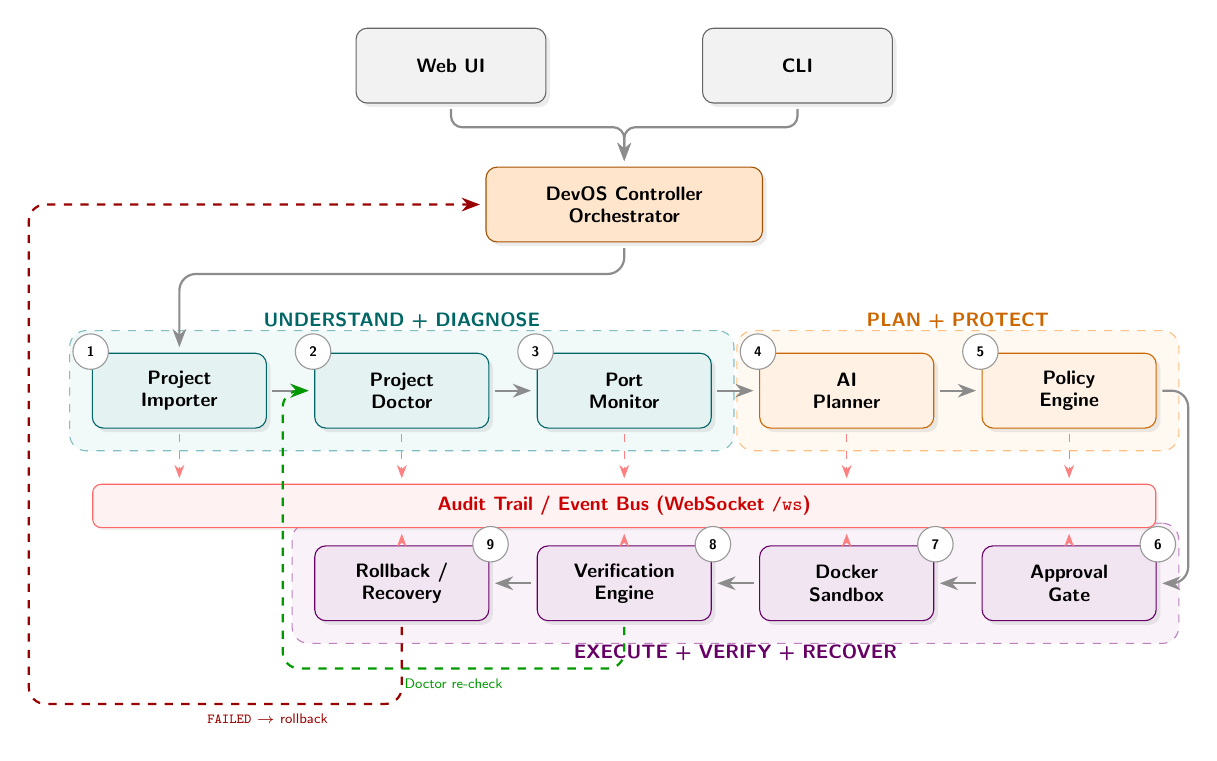
\begin{tikzpicture}[
    >=Stealth,
    font=\sffamily\footnotesize,
    % --- Node styles ---
    box/.style={
        rectangle, draw=#1!80!black, fill=#1!10,
        rounded corners=4pt, minimum height=0.95cm,
        minimum width=2.1cm, text centered,
        text width=2.0cm, inner sep=3pt,
        font=\sffamily\scriptsize\bfseries,
        drop shadow={opacity=0.15, shadow xshift=1.5pt, shadow yshift=-1.5pt}
    },
    box/.default=gray,
    stepnum/.style={
        circle, draw=gray!80, fill=white,
        font=\sffamily\bfseries\tiny, inner sep=1pt,
        minimum size=0.45cm
    },
    mainflow/.style={->, thick, color=gray!90, shorten >=2pt, shorten <=2pt},
    feedback/.style={->, thick, dashed, shorten >=2pt, shorten <=2pt},
    auditline/.style={->, thin, dashed, draw=red!50, shorten >=2pt, shorten <=2pt},
    phaselabel/.style={font=\sffamily\bfseries\scriptsize, text=#1!80!black},
    phaselabel/.default=blue
]

% ========== TOP ROW (L to R) ==========
\node[box=teal] (monitor) {\textbf{Port}\\\textbf{Monitor}};
\node[box=teal, left=0.6cm of monitor] (doctor) {\textbf{Project}\\\textbf{Doctor}};
\node[box=teal, left=0.6cm of doctor] (importer) {\textbf{Project}\\\textbf{Importer}};
\node[box=orange, right=0.6cm of monitor] (planner) {\textbf{AI}\\\textbf{Planner}};
\node[box=orange, right=0.6cm of planner] (policy) {\textbf{Policy}\\\textbf{Engine}};

% ========== EVENT BUS (Middle) ==========
\node[rectangle, draw=red!60, fill=red!5, rounded corners=3pt,
      minimum width=13.5cm, minimum height=0.55cm,
      below=0.7cm of monitor,
      font=\sffamily\scriptsize\bfseries, text=red!80!black,
      drop shadow={opacity=0.1, shadow xshift=1pt, shadow yshift=-1pt}]
      (audit) {Audit Trail / Event Bus (WebSocket \texttt{/ws})};

% ========== BOTTOM ROW (R to L) ==========
\coordinate (bottom_y) at ($(audit.south) - (0, 0.7cm)$);
\node[box=violet] (approval) at (policy |- bottom_y) {\textbf{Approval}\\\textbf{Gate}};
\node[box=violet] (sandbox)  at (planner |- bottom_y) {\textbf{Docker}\\\textbf{Sandbox}};
\node[box=violet] (verify)   at (monitor |- bottom_y) {\textbf{Verification}\\\textbf{Engine}};
\node[box=violet] (rollback) at (doctor |- bottom_y) {\textbf{Rollback /}\\\textbf{Recovery}};

% ========== CONTROLLER & UI (Top) ==========
\node[box=orange!80!black, fill=orange!20, minimum width=3.5cm, text width=3.3cm,
      above=1.4cm of monitor]
      (controller) {\textbf{DevOS Controller}\\Orchestrator};

\node[box=gray, above=0.8cm of controller, xshift=-2.2cm, minimum width=2.4cm, text width=2.2cm] (webui) {\textbf{Web UI}};
\node[box=gray, above=0.8cm of controller, xshift=2.2cm, minimum width=2.4cm, text width=2.2cm] (cli) {\textbf{CLI}};

% ========== MAIN FLOW ARROWS ==========
\draw[mainflow] (importer) -- (doctor);
\draw[mainflow] (doctor) -- (monitor);
\draw[mainflow] (monitor) -- (planner);
\draw[mainflow] (planner) -- (policy);

% Turn around the right side
\draw[mainflow, rounded corners=6pt] (policy.east) -- ++(0.4,0) |- (approval.east);

\draw[mainflow] (approval) -- (sandbox);
\draw[mainflow] (sandbox) -- (verify);
\draw[mainflow] (verify) -- (rollback);

% UI down to Controller
\draw[mainflow, rounded corners=4pt] (webui.south) -- ++(0,-0.3) -| (controller.north);
\draw[mainflow, rounded corners=4pt] (cli.south) -- ++(0,-0.3) -| (controller.north);

% Controller down to Importer
\draw[mainflow, rounded corners=6pt] (controller.south) -- ++(0,-0.4) -| (importer.north);

% ========== FEEDBACK LOOPS ==========
% Verify to Doctor (Green)
\draw[feedback, color=green!60!black, rounded corners=6pt]
    (verify.south) -- ++(0, -0.6) -|
    node[pos=0.25, below, font=\sffamily\tiny, color=green!60!black] {Doctor re-check}
    ($(rollback.west)+(-0.4, 0)$) |- (doctor.west);

% Rollback to Controller (Red)
\draw[feedback, color=red!60!black, rounded corners=6pt]
    (rollback.south) -- ++(0, -1.05) -|
    node[pos=0.18, below, font=\sffamily\tiny, color=red!60!black] {\texttt{FAILED} $\to$ rollback}
    ($(importer.west)+(-0.8, 0)$) |- (controller.west);

% ========== AUDIT LINES ==========
\foreach \n in {importer, doctor, monitor, planner, policy} {
    \draw[auditline] (\n.south) -- (\n.south |- audit.north);
}
\foreach \n in {approval, sandbox, verify, rollback} {
    \draw[auditline] (\n.north) -- (\n.north |- audit.south);
}

% ========== GROUPING BOXES ==========
\begin{scope}[on background layer]
    \node[fit=(importer)(doctor)(monitor),
          draw=teal!50, fill=teal!5, dashed, rounded corners=6pt, inner sep=8pt,
          label={[phaselabel=teal, yshift=-3pt]above:{\textsf{UNDERSTAND + DIAGNOSE}}}] {};
    \node[fit=(planner)(policy),
          draw=orange!50, fill=orange!5, dashed, rounded corners=6pt, inner sep=8pt,
          label={[phaselabel=orange, yshift=-3pt]above:{\textsf{PLAN + PROTECT}}}] {};
    \node[fit=(approval)(sandbox)(verify)(rollback),
          draw=violet!50, fill=violet!5, dashed, rounded corners=6pt, inner sep=8pt,
          label={[phaselabel=violet, yshift=3pt]below:{\textsf{EXECUTE + VERIFY + RECOVER}}}] {};
\end{scope}

% ========== STEP NUMBERS ==========
\node[stepnum, above left=-0.15cm and -0.15cm of importer.north west] {1};
\node[stepnum, above left=-0.15cm and -0.15cm of doctor.north west] {2};
\node[stepnum, above left=-0.15cm and -0.15cm of monitor.north west] {3};
\node[stepnum, above left=-0.15cm and -0.15cm of planner.north west] {4};
\node[stepnum, above left=-0.15cm and -0.15cm of policy.north west] {5};
\node[stepnum, above right=-0.15cm and -0.15cm of approval.north east] {6};
\node[stepnum, above right=-0.15cm and -0.15cm of sandbox.north east] {7};
\node[stepnum, above right=-0.15cm and -0.15cm of verify.north east] {8};
\node[stepnum, above right=-0.15cm and -0.15cm of rollback.north east] {9};

\end{tikzpicture}
\caption{DevOS self-healing pipeline. Numbered steps show the data flow: the Controller dispatches to diagnostic probes (\circled{1}--\circled{3}), the rule-based Planner and Policy Engine gate actions (\circled{4}--\circled{5}), the Approval UI presents risky actions to the developer (\circled{6}), the Docker Sandbox executes in isolation (\circled{7}), the Verification Engine runs a multi-layer health ladder (\circled{8}), and Rollback restores state on failure (\circled{9}). Green dashed line: Doctor re-check loop. Red dashed line: \texttt{FAILED} verdict triggers state rollback. All steps emit to the central Audit Event Bus.}
\label{fig:architecture}
\end{figure*}

\subsubsection{Project Importer (Understand)}
The \texttt{Importer} service builds a \textit{Project Manifest} from a filesystem path:
\begin{itemize}[leftmargin=*, nosep]
    \item \textbf{Stack Detection:} \texttt{package.json} (Node/npm), \texttt{requirements.txt}/\texttt{pyproject.toml} (Python), \texttt{go.mod} (Go), \texttt{Cargo.toml} (Rust).
    \item \textbf{Configuration:} \texttt{.env.example} vs \texttt{.env} diff; masked secret values.
    \item \textbf{Dependencies:} Declared vs. installed (\texttt{node\_modules}, \texttt{venv}).
    \item \textbf{Ports:} Configured \texttt{PORT} from code/config.
    \item \textbf{Database:} \texttt{db/*.sql} files $\to$ table list; compose services.
    \item \textbf{Commands:} \texttt{start}, \texttt{build}, \texttt{test}, \texttt{dev} from \texttt{package.json} scripts.
    \item \textbf{Git:} Status, branch, uncommitted changes, recent commits.
\end{itemize}
Re-importing a path reuses the newest \texttt{Project} record (idempotent).

\subsubsection{Project Doctor (Diagnose)}
\label{sec:doctor}
The \texttt{Doctor} runs read-only \textit{probes} against the real machine and applies pure diagnostic rules:
\begin{itemize}[leftmargin=*, nosep]
    \item \textbf{Probes:} Port bind test (dual-stack \texttt{::} like Node), \texttt{psutil} process holder, PostgreSQL connectivity via \texttt{psycopg} (error classification: unreachable/auth/missing-DB), sandboxed app start (captures crash output).
    \item \textbf{Finding Types:} \texttt{env\_missing}, \texttt{dependency\_missing}, \texttt{port\_in\_use}, \texttt{database\_unreachable}, \texttt{database\_auth}, \texttt{schema\_missing}, \texttt{runtime\_crash}.
    \item \textbf{Ranking:} Priority = Severity Weight $\times$ Confidence. If \texttt{.env} lacks \texttt{DATABASE\_URL}, the DB is probed via \texttt{.env.example} so one gap cannot hide a second problem.
\end{itemize}

\subsubsection{AI Planner (Plan)}
\label{sec:planner}
The planner uses a \textbf{closed rule table} (\texttt{planner.RULES}) mapping finding types to ordered action sequences. Algorithm~\ref{alg:planner} formalizes the planning process.

\begin{algorithm}[t]
\caption{Deterministic Recovery Planning}
\label{alg:planner}
\small
\begin{algorithmic}[1]
\Require Findings $F = \{f_1, \ldots, f_n\}$ ranked by priority
\Require Rule table $R: \text{FindingType} \to \text{ActionSequence}$
\Require Tier ordering $T = [\text{settings}, \text{packages}, \text{port}, \text{db\_start}, \text{db\_login}, \text{migration}]$
\Ensure Recovery plan $P = [a_1, \ldots, a_m]$
\State $P \gets []$
\For{each tier $t \in T$}
    \For{each finding $f \in F$ where $\text{tier}(R[f.\text{type}]) = t$}
        \State $actions \gets R[f.\text{type}].\text{instantiate}(f.\text{evidence})$
        \For{each $a \in actions$}
            \State $a.\text{risk} \gets \text{Policy.classify}(a.\text{type})$
            \If{$a.\text{risk} \neq \texttt{BLOCK}$}
                \State $P.\text{append}(a)$
            \EndIf
        \EndFor
    \EndFor
\EndFor
\If{LLM key available}
    \State $P \gets \text{LLM\_explain}(P)$ \Comment{Adds explanations only}
    \State $P \gets \text{LLM\_review}(P)$ \Comment{Reorders within tiers only}
\EndIf
\State \Return $P$
\end{algorithmic}
\end{algorithm}

Tiers enforce a fixed ordering: settings $\to$ packages $\to$ port $\to$ DB start $\to$ DB login $\to$ migration. This ensures dependencies between repair actions are respected (\eg the database must be reachable before running a migration).

\textbf{LLM Role (Optional):} Only writes a one-sentence explanation per step in a strict JSON schema. Cannot add/drop/reorder steps across tiers. Fallback to rule text on any failure. Audit records \texttt{planner:llm} or \texttt{planner:rules}.

\subsubsection{Plan Review (AI Cross-Check)}
\label{sec:plan-review}
With an LLM key, a second model \textit{reviews} the rule-generated plan: outputs \texttt{agree/doubt}, note, score (0--100), and \texttt{missing} check names. Deterministic \textit{cross-check} verifies each step: (1) rule reproduces action, (2) policy $\neq$ \texttt{BLOCK}, (3) covered by \texttt{targets\_of} (verification can re-check). Failing steps are \textit{excluded} before storage. Ranking: AI score reorders only \textit{within a tier}; tier order is invariant.

\subsubsection{Policy Engine \& Approval (Protect)}
\label{sec:policy}
Each \texttt{ActionType} has a fixed \texttt{RiskLevel} and \texttt{PolicyDecision} (see \texttt{policy.py}, Appendix~\ref{app:actions}):
\begin{itemize}[leftmargin=*, nosep]
    \item \texttt{ALLOW}: \texttt{read\_file}, \texttt{run\_build}, \texttt{run\_tests}
    \item \texttt{REQUIRE\_APPROVAL}: \texttt{set\_env\_var}, \texttt{install\_dependency}, \texttt{restart\_service}, \texttt{write\_file}, \texttt{free\_port}, \texttt{run\_migration}
    \item Default deny: any unknown \texttt{ActionType} is blocked automatically
\end{itemize}
The UI shows issue, evidence, proposed action, risk, and \textit{can't-undo} warnings before approval. This policy layer is what distinguishes \devos from autonomous SWE agents~\cite{swe-agent, devin}: the AI never acts without a human gate for risky operations.

\subsubsection{Docker Sandbox (Execute)}
\label{sec:sandbox}
Approved actions execute in the \texttt{devos-sandbox} image (content-tagged by \texttt{Dockerfile} + \texttt{runner.js} hash):
\begin{itemize}[leftmargin=*, nosep]
    \item \textbf{Limits (defaults):} 1 CPU, 512 MB RAM, 300 s timeout, \texttt{/work} (project) RW, read-only root filesystem, no network except \texttt{install\_dependency}/\texttt{run\_migration}.
    \item \textbf{Runner:} \texttt{sandbox/runner.js} dispatches fixed handlers; request parameters \textit{never} become CLI args. Unknown types $\to$ fail closed.
    \item \textbf{Actions Implemented:} \texttt{set\_env\_var}, \texttt{install\_dependency}, \texttt{run\_migration}, \texttt{restart\_service}, \texttt{read\_file}.
\end{itemize}

\subsubsection{Verification Engine (Verify)}
\label{sec:verification}
Layered verification (sequential; stop on failure):
\begin{enumerate}[leftmargin=*, nosep]
    \item \textbf{Sandbox Health:} App starts + answers \texttt{/health} in sandbox.
    \item \textbf{Build:} Project \texttt{build} script (if defined).
    \item \textbf{Test:} Project \texttt{test} script (if defined).
    \item \textbf{Log Review:} Sandbox logs scanned for errors.
    \item \textbf{Doctor Re-check:} Full \texttt{Doctor} run; every targeted finding (matched by check + setting) must be gone (retries for just-started DB).
\end{enumerate}
\textbf{Verdicts:} \texttt{VERIFIED} (all pass), \texttt{PARTIALLY VERIFIED} (failing tests/logs but targeted problems gone), \texttt{FAILED} (won't start, build fails, targeted problem remains $\to$ rollback), \texttt{NOT TESTED} (sandbox/infra failure).

This multi-layer approach contrasts with SWE-bench agents that rely solely on test-suite pass/fail~\cite{swe-bench} and with self-healing infrastructure that checks only liveness/readiness probes~\cite{k8s-operators}.

\subsubsection{Rollback/Recovery (Recover)}
\label{sec:rollback}
Pre-execution snapshot of project files (excludes \texttt{node\_modules}, \texttt{.git}). On \texttt{FAILED}: restore files. \textbf{Explicit non-undoable:} installed packages, applied migrations, started services (listed in \texttt{executor.NOT\_UNDONE}, surfaced in UI/log).

\subsubsection{Audit Trail (Cross-Cutting)}
\label{sec:audit}
\texttt{pipeline.py} orchestrates and emits \texttt{AuditEvent} per state change: \texttt{project\_imported}, \texttt{diagnosis\_completed}, \texttt{plan\_generated}, \texttt{plan\_approved}, \texttt{execution\_started}, \texttt{execution\_completed}, \texttt{verification\_completed}, \texttt{rollback\_executed}. WebSocket (\texttt{/ws}) pushes live progress. This follows the observability-by-default principle of autonomic computing~\cite{autonomic2001}.

\subsection{Reference Implementation}
\label{sec:implementation}
\begin{itemize}[leftmargin=*, nosep]
    \item \textbf{Backend:} Python 3.11+, FastAPI, SQLAlchemy, PostgreSQL (DevOS's own DB), \texttt{psycopg}, \texttt{psutil}, Docker SDK, Pytest (245 tests).
    \item \textbf{Frontend:} React 18, TypeScript, Vite, \texttt{@nuxt/ui} components, WebSocket client.
    \item \textbf{CLI:} \texttt{typer} + \texttt{rich} + \texttt{httpx} (\texttt{devos doctor|fix|up|status|audit}).
    \item \textbf{Sandbox:} \texttt{node:20-alpine} base, \texttt{runner.js} fixed dispatcher.
    \item \textbf{Demo App:} React + Express + PostgreSQL (port 5433), \texttt{db/schema.sql}, own \texttt{docker-compose.yml}, 8 injectable failure modes.
    \item \textbf{Scripts:} \texttt{dev.py} (one-command start), \texttt{inject\_failure.py}, \texttt{run\_scenarios.py}, \texttt{run\_demo.py}.
\end{itemize}

% ==============================================================================
% 4. RESULTS AND DISCUSSION
% ==============================================================================
\section{Results and Discussion}
\label{sec:results}

\subsection{Experimental Setup}
All experiments run on a developer laptop (Intel i7, 16 GB RAM, Docker Desktop/WSL2). The DevOS backend, frontend, and its PostgreSQL run via \texttt{python scripts/dev.py}. The demo app runs in the sandbox. Nine scenarios from \texttt{run\_scenarios.py} exercise the full pipeline against real Docker/Postgres.

\subsection{Scenario Results}
Table~\ref{tab:scenarios} summarizes the nine end-to-end scenarios. All reparable scenarios achieve \texttt{VERIFIED}; the unfixable scenario correctly yields \texttt{FAILED} with automatic rollback.

\begin{table*}[t]
\centering
\caption{End-to-End Scenario Results (\texttt{run\_scenarios.py})}
\label{tab:scenarios}
\small
\renewcommand{\arraystretch}{1.15}
\begin{tabular*}{\linewidth}{@{\extracolsep{\fill}}llclc@{}}
\toprule
\textbf{Scenario} & \textbf{Injected Failures} & \textbf{Steps} & \textbf{Verdict} & \textbf{Rollback} \\
\midrule
\texttt{missing-env} & \texttt{DATABASE\_URL} missing & 1 & \vpass & No \\
\texttt{missing-dependency} & \texttt{node\_modules} deleted & 1 & \vpass & No \\
\texttt{port-conflict} & Port holder on configured PORT & 1 & \vpass & No \\
\texttt{db-down} & Demo Postgres stopped & 1 & \vpass & No \\
\texttt{db-auth} & Wrong password in \texttt{.env} & 1 & \vpass & No \\
\texttt{db-schema} & Tables missing & 1 & \vpass & No \\
\texttt{combo} & \texttt{missing-env} + \texttt{db-down} + \texttt{db-auth} & 3 & \vpass & No \\
\texttt{crash} & Syntax error in app code & 0 & \vna\ (diagnosis only) & N/A \\
\texttt{unfixable} & Bad \texttt{.env.example} default & 1 & \vfail & \checkmark \\
\bottomrule
\end{tabular*}
\end{table*}

\subsection{Qualitative Analysis}

\subsubsection{Missing Environment Variable (\texttt{missing-env})}
\devos detects \texttt{DATABASE\_URL} absent from \texttt{.env} but present in \texttt{.env.example}. Plan: \texttt{set\_env\_var(DATABASE\_URL=...)}. Sandbox writes \texttt{.env}, app starts, \texttt{/health} returns 200, Doctor re-check passes. Verdict: \vpass.

\subsubsection{Port Conflict (\texttt{port-conflict})}
A holder process binds the configured port. \devos detects \texttt{port\_in\_use} (probe binds dual-stack \texttt{::} like Node). Plan: \texttt{set\_env\_var(PORT=<free>)}. App starts on new port. Verdict: \vpass. \textit{Note:} DevOS \textit{changes the port setting} (undoable), never kills the holder (\texttt{free\_port} is \texttt{BLOCK}). This design choice---prefer the reversible action over the destructive one---exemplifies the safety-by-construction principle.

\subsubsection{Database Down (\texttt{db-down})}
Demo compose service \texttt{db} is stopped. \devos detects \texttt{database\_unreachable}. Plan: \texttt{restart\_service(devos-demo-db)}. Docker API starts container; retries handle Postgres startup delay. Doctor re-check confirms connectivity. Verdict: \vpass.

\subsubsection{Combined Multi-Failure (\texttt{combo})}
Three simultaneous failures: missing \texttt{DATABASE\_URL}, stopped DB, wrong password. \devos produces a 3-step plan (settings $\to$ DB start $\to$ login). Steps execute sequentially; each verified before next. All three findings resolved. Verdict: \vpass. Demonstrates \textit{tier ordering} (settings before DB before login) and \textit{dependency-aware probing} (probes DB via \texttt{.env.example} before \texttt{.env} is fixed).

\subsubsection{Unfixable Failure (\texttt{unfixable})}
\texttt{.env.example} itself contains an invalid default. \devos sets \texttt{DATABASE\_URL} from \texttt{.env.example}, but DB connection fails. Verification: Doctor re-check finds \texttt{database\_auth} still present $\to$ \vfail. Rollback restores original \texttt{.env}. UI shows \vfail\ verdict, rollback log, and \textit{non-undoable} note (none here). Demonstrates \textit{safety}: a bad fix is caught and reverted automatically---a capability absent from both AI coding assistants and SWE agents.

\subsection{Comparison with Autonomous Agents}
\label{sec:agent-comparison}
DevOS and autonomous SWE agents~\cite{swe-agent, autocoderover, devin} are \textit{complementary}, not competing. To illustrate the distinction:

\begin{itemize}[leftmargin=*, nosep]
    \item A SWE agent given a GitHub issue ``fix the null pointer in \texttt{user\_service.py}'' navigates the codebase, writes a patch, and verifies via tests---\textit{inside a pre-configured Docker container}.
    \item \devos given a broken project detects that \texttt{DATABASE\_URL} is missing, PostgreSQL is stopped, and the schema is un-migrated---\textit{before any code-level tool can run}.
\end{itemize}

The ideal pipeline is: \devos heals the environment $\to$ SWE agent fixes the code $\to$ \devos verifies the result.

\subsection{Performance \& Resource Usage}
\begin{itemize}[leftmargin=*, nosep]
    \item \textbf{Import + Diagnose:} $\sim$2--5 s (probes dominate: port bind, DB connect, sandbox start).
    \item \textbf{Plan Generation:} $\sim$50--200 ms (rules); +1--3 s if LLM explanation enabled (API latency).
    \item \textbf{Sandbox Execution:} $\sim$5--30 s per step (\texttt{npm install} dominates at $\sim$15--25 s cold).
    \item \textbf{Verification:} $\sim$10--20 s (health + build + test + Doctor re-check).
    \item \textbf{Total Loop (combo):} $\sim$60--90 s end-to-end.
    \item \textbf{Sandbox Limits Effective:} CPU/memory enforcement verified via \texttt{docker stats}; network isolation verified (no external egress except allowlisted actions).
\end{itemize}

\subsection{Test Coverage}
\begin{itemize}[leftmargin=*, nosep]
    \item \textbf{Backend:} 245 tests (unit + integration). DB-backed tests use savepoint rollback. Docker tests skip if daemon unavailable. \texttt{probes.collect} stubbed in \texttt{conftest.py} for isolation.
    \item \textbf{Frontend:} TypeScript build (\texttt{npm run build}) passes; manual UI verification + scripted browser via \texttt{run\_scenarios.py}.
    \item \textbf{E2E:} \texttt{run\_scenarios.py} drives real API + real Docker; 9/9 scenarios pass.
\end{itemize}

\subsection{Limitations}
\label{sec:limitations}
\begin{enumerate}[leftmargin=*, nosep]
    \item \textbf{Single Reference Stack:} React + Node.js + PostgreSQL only. No Python, Go, Java, MySQL, MongoDB, \etc
    \item \textbf{No Code-Level Repair:} \texttt{runtime\_crash} and \texttt{database\_missing} are diagnosis-only. Integrating an LLM-based APR tool~\cite{llm-apr-survey-2025} for code fixes is future work.
    \item \textbf{No Background Job Queue:} FastAPI \texttt{BackgroundTasks} only; no persistence across restarts.
    \item \textbf{No Authentication/Multi-User:} Localhost-only API by design.
    \item \textbf{File-Only Rollback:} Cannot undo installed packages, applied migrations, started services.
    \item \textbf{Doctor Gaps:} No Git health checks, dependency version mismatch detection, docker-compose health checks, other DB kinds.
    \item \textbf{No SWE-bench Evaluation:} DevOS addresses \textit{environment} failures, not \textit{code} bugs, so SWE-bench is not directly applicable. A custom benchmark for environment healing is needed.
\end{enumerate}

% ==============================================================================
% 5. CONCLUSION
% ==============================================================================
\section{Conclusion}
\label{sec:conclusion}

We presented \devos, a self-healing AI development environment that automates the full recovery loop for broken software projects: \textbf{Understand $\to$ Diagnose $\to$ Protect $\to$ Execute $\to$ Verify $\to$ Recover}. Unlike AI coding assistants that generate code with unrestricted shell access, and unlike autonomous SWE agents~\cite{swe-agent, devin} that assume a pre-configured environment, \devos focuses on \textit{environmental healing}---configuration, dependencies, ports, databases, services---with safety guarantees at every stage: deterministic rule-based planning, policy-gated actions, mandatory approval, sandboxed execution with resource bounds, layered verification, and automatic rollback.

Our prototype demonstrates the loop on a React/Node/PostgreSQL reference stack, automatically repairing eight failure classes across nine end-to-end scenarios with 100\% success on reparable failures and correct rollback on the unverifiable case. The system is implemented in $\sim$15k lines of Python/TypeScript, with 245 backend tests, a three-pane web UI, and a terminal CLI.

\textbf{Future Work:}
\begin{enumerate}[leftmargin=*, nosep]
    \item Generalizing to multiple language/framework stacks (Python/pip, Go/modules, Rust/Cargo).
    \item Integrating LLM-based code repair~\cite{llm-apr-survey-2025} for \texttt{runtime\_crash} findings, with the same policy--sandbox--verify--rollback chain.
    \item Implementing a persistent job queue (Celery/Redis) for production-grade orchestration.
    \item Adding Alembic migrations for DevOS's own schema evolution.
    \item CI integration for \texttt{run\_scenarios.py} as a regression suite.
    \item Richer monitoring (per-project CPU/memory via cgroups).
    \item Diff-aware database rollback via snapshots.
    \item Creating a dedicated \textit{environment healing benchmark} analogous to SWE-bench for code repair.
\end{enumerate}

% ==============================================================================
% APPENDIX
% ==============================================================================
\appendices

\section{Action Type Definitions}
\label{app:actions}
Table~\ref{tab:actions} lists all nine \texttt{ActionType} enum members from \texttt{domain/enums.py} with their risk level and policy decision as defined in \texttt{services/policy.py}. Actions without a matching rule are blocked by default (``default deny'').

\begin{table}[h!]
\centering
\caption{Implemented Action Types and Policies (from \texttt{policy.py})}
\label{tab:actions}
\renewcommand{\arraystretch}{1.4} % Adds breathing room
\begin{tabularx}{\linewidth}{@{} l X c c @{}}
\toprule
\textbf{Action Type} & \textbf{Description} & \textbf{Risk} & \textbf{Policy} \\
\midrule
\texttt{read\_file}          & Read project file (size-capped)    & \badgeLow  & \badgeAllow \\
\texttt{run\_build}          & Run project build script           & \badgeLow  & \badgeAllow \\
\texttt{run\_tests}          & Run project test suite             & \badgeLow  & \badgeAllow \\
\midrule
\texttt{set\_env\_var}       & Write key=value to \texttt{.env}   & \badgeMed  & \badgeReq \\
\texttt{install\_dependency} & \texttt{npm install} (scripts off) & \badgeMed  & \badgeReq \\
\texttt{restart\_service}    & \texttt{docker compose up -d}      & \badgeMed  & \badgeReq \\
\texttt{write\_file}         & Write/edit project file            & \badgeMed  & \badgeReq \\
\texttt{free\_port}          & Kill process on port               & \badgeHigh & \badgeReq \\
\texttt{run\_migration}      & Execute \texttt{.sql} in trans.    & \badgeHigh & \badgeReq \\
\midrule
\textit{(unknown type)}      & Not in \texttt{ActionType} enum    & \badgeHigh & \badgeBlock \\
\bottomrule
\end{tabularx}
\vspace{4pt}
\raggedright\scriptsize \textit{Note:} Path-escape check: any action with a \texttt{path} parameter that is absolute or contains \texttt{..} is blocked regardless of its risk level.
\end{table}

\vspace{1em}
\section{Finding Type Definitions}
\label{app:findings}
\begin{table}[h!]
\centering
\caption{Project Doctor Finding Types}
\label{tab:findings}
\small
\begin{tabular}{@{}llc@{}}
\toprule
\textbf{Finding Type} & \textbf{Description} & \textbf{Fixable} \\
\midrule
\texttt{env\_missing}           & Required key absent from \texttt{.env}               & \checkmark \\
\texttt{dependency\_missing}    & \texttt{node\_modules} incomplete                     & \checkmark \\
\texttt{port\_in\_use}          & Configured port held by another process              & \checkmark \\
\texttt{database\_unreachable}  & Postgres host/port not accepting connections          & \checkmark \\
\texttt{database\_auth}         & Credentials rejected                                  & \checkmark \\
\texttt{schema\_missing}        & Tables from \texttt{db/*.sql} not found               & \checkmark \\
\midrule
\texttt{runtime\_crash}         & App process exits with error                          & \ding{55} (diagnosis only) \\
\texttt{database\_missing}      & Database does not exist                               & \ding{55} (diagnosis only) \\
\bottomrule
\end{tabular}
\end{table}

\vspace{1em}
\section{MAPE-K Loop Mapping}
\label{app:mapek}
Table~\ref{tab:mapek} maps DevOS's pipeline to the classical autonomic computing MAPE-K reference model~\cite{autonomic2001}, showing how each phase corresponds to the self-healing control loop.

\begin{table}[h!]
\centering
\caption{DevOS Pipeline Mapped to MAPE-K}
\label{tab:mapek}
\small
\begin{tabular}{@{}lll@{}}
\toprule
\textbf{MAPE-K Phase} & \textbf{DevOS Component} & \textbf{Artifacts} \\
\midrule
Monitor  & Importer, Port Monitor  & Manifest, port map \\
Analyze  & Project Doctor          & Ranked findings \\
Plan     & AI Planner + Review     & Typed action plan \\
Execute  & Policy $\to$ Sandbox    & Execution results \\
Knowledge & Audit Trail            & Event log \\
\bottomrule
\end{tabular}
\end{table}

% ==============================================================================
% REFERENCES
% ==============================================================================
\balance  % Balance columns on last page (IEEE requirement)
\bibliographystyle{IEEEtran}
\bibliography{references}

\end{document}